% Seminar 1: Procese Stochastice și Staționaritate
% Prezentare academică de calitate Harvard
% Program de licență, Academia de Studii Economice din București

\documentclass[9pt, aspectratio=169, t]{beamer}

% Asigură încadrarea conținutului pe diapozitive
\setbeamersize{text margin left=8mm, text margin right=8mm}

%=============================================================================
% CONFIGURARE TEMĂ ȘI STIL
%=============================================================================
\usetheme{default}
% Using default theme for clean header/footer control

% Color Palette (matching Redispatch PDF)
\definecolor{MainBlue}{RGB}{26, 58, 110}
\definecolor{AccentBlue}{RGB}{26, 58, 110}
\definecolor{IDAred}{RGB}{205, 0, 0}
\definecolor{DarkGray}{RGB}{51, 51, 51}
\definecolor{MediumGray}{RGB}{128, 128, 128}
\definecolor{LightGray}{RGB}{248, 248, 248}
\definecolor{VeryLightGray}{RGB}{235, 235, 235}
\definecolor{KeynoteGray}{RGB}{218, 218, 218}
\definecolor{SectionGray}{RGB}{120, 120, 120}
\definecolor{FooterGray}{RGB}{100, 100, 100}
\definecolor{Crimson}{RGB}{220, 53, 69}
\definecolor{Forest}{RGB}{46, 125, 50}
\definecolor{Amber}{RGB}{181, 133, 63}
\definecolor{Orange}{RGB}{230, 126, 34}
\definecolor{Purple}{RGB}{142, 68, 173}

% Gradient background (exact Keynote 315° gradient: white to RGB 218,218,218)
\setbeamertemplate{background}{%
    \begin{tikzpicture}[remember picture, overlay]
        \shade[shading=axis, shading angle=315,
        top color=white, bottom color=KeynoteGray]
        (current page.south west) rectangle (current page.north east);
    \end{tikzpicture}%
}
% Fallback solid color for compatibility
\setbeamercolor{background canvas}{bg=}

\setbeamercolor{palette primary}{bg=MainBlue, fg=white}
\setbeamercolor{palette secondary}{bg=MainBlue!85, fg=white}
\setbeamercolor{palette tertiary}{bg=MainBlue!70, fg=white}
\setbeamercolor{structure}{fg=MainBlue}
\setbeamercolor{title}{fg=IDAred}
\setbeamercolor{frametitle}{fg=IDAred, bg=}
\setbeamercolor{block title}{bg=MainBlue, fg=white}
\setbeamercolor{block body}{bg=VeryLightGray, fg=DarkGray}
\setbeamercolor{block title alerted}{bg=Crimson, fg=white}
\setbeamercolor{block body alerted}{bg=Crimson!8, fg=DarkGray}
\setbeamercolor{block title example}{bg=Forest, fg=white}
\setbeamercolor{block body example}{bg=Forest!8, fg=DarkGray}
\setbeamercolor{item}{fg=MainBlue}

% Footer colors (override Madrid theme blue)
\setbeamercolor{author in head/foot}{fg=FooterGray, bg=}
\setbeamercolor{title in head/foot}{fg=FooterGray, bg=}
\setbeamercolor{date in head/foot}{fg=FooterGray, bg=}
\setbeamercolor{section in head/foot}{fg=FooterGray, bg=}
\setbeamercolor{subsection in head/foot}{fg=FooterGray, bg=}

% Bullet styles (apply everywhere including blocks)
\setbeamertemplate{itemize item}{\color{MainBlue}$\boxdot$}
\setbeamertemplate{itemize subitem}{\color{MainBlue}$\blacktriangleright$}
\setbeamertemplate{itemize subsubitem}{\color{MainBlue}\tiny$\bullet$}
\setbeamertemplate{itemize/enumerate body begin}{\normalsize}
\setbeamertemplate{itemize/enumerate subbody begin}{\normalsize}

% Item spacing - compact style
\setlength{\leftmargini}{10pt}       % Level 1: minimal indent
\setlength{\leftmarginii}{10pt}      % Level 2: minimal additional indent
% Compact list spacing (zero extra space before/after lists in blocks)
\makeatletter
\def\@listi{\leftmargin\leftmargini \topsep 0pt \parsep 0pt \itemsep 0pt}
\def\@listii{\leftmargin\leftmarginii \topsep 0pt \parsep 0pt \itemsep 0pt}
\makeatother

\setbeamertemplate{navigation symbols}{}

%=============================================================================
% CUSTOM HEADLINE
%=============================================================================
\setbeamertemplate{headline}{%
    \vskip10pt%
    \hbox to \paperwidth{%
        \hskip0.5cm%
        {\small\color{FooterGray}\renewcommand{\hyperlink}[2]{##2}\insertsectionhead}%
        \hfill%
        \textcolor{FooterGray}{\small\insertframenumber}%
        \hskip0.5cm%
    }%
    \vskip4pt%
    {\color{FooterGray}\hrule height 0.4pt}%
}

%=============================================================================
% CUSTOM FOOTER
%=============================================================================
\usepackage{fontawesome5}

\setbeamertemplate{footline}{%
    {\color{FooterGray}\hrule height 0.4pt}%
    \vskip4pt%
    \hbox to \paperwidth{%
        \hskip0.5cm%
        \textcolor{FooterGray}{\small Analiza și Prognoza seriilor de timp}%
        \hfill%
        \raisebox{-0.1em}{%
            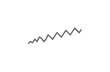
\begin{tikzpicture}[x=0.08em, y=0.08em, line width=0.4pt]
                \draw[FooterGray] (0,3) -- (1,4) -- (2,3.5) -- (3,5) -- (4,4) -- (5,6) -- (6,5.5) -- (7,4) -- (8,5) -- (9,7) -- (10,6) -- (11,5) -- (12,6.5) -- (13,8) -- (14,7) -- (15,6) -- (16,7.5) -- (17,9) -- (18,8) -- (19,7) -- (20,8.5) -- (21,10) -- (22,9) -- (23,8) -- (24,9.5);
            \end{tikzpicture}%
        }%
        \hskip0.5cm%
    }%
    \vskip6pt%
}

%=============================================================================
% PACHETE
%=============================================================================
\usepackage[utf8]{inputenc}
\usepackage[T1]{fontenc}
\usepackage[romanian]{babel}
\usepackage{amsmath, amssymb, amsthm}
\usepackage{mathtools}
\usepackage{bm}
\usepackage{tikz}
\usetikzlibrary{arrows.meta, positioning, shapes, calc, decorations.pathreplacing, shadings}
\usepackage{booktabs}
\usepackage{multirow}
\usepackage{array}
\usepackage{graphicx}
\usepackage{hyperref}
\usepackage{colortbl}
\hypersetup{colorlinks=true, linkcolor=MainBlue, urlcolor=MainBlue}
\graphicspath{{../../logos/}{../../charts/}}
\hfuzz=2pt  % Suppress tiny overfull warnings (<2pt)
\vfuzz=2pt  % Suppress tiny vertical overfull warnings (<2pt)

%=============================================================================
% COMANDA QUANTLET
%=============================================================================
\newcommand{\quantlet}[2]{%
    \hfill\href{#2}{%
        \raisebox{-0.15em}{\includegraphics[height=0.7em]{ql_logo.png}}%
        \textcolor{MainBlue}{\tiny\ #1}%
    }%
}

%=============================================================================
% COMENZI PERSONALIZATE
%=============================================================================
\newcommand{\E}{\mathbb{E}}
\newcommand{\Var}{\text{Var}}
\newcommand{\Cov}{\text{Cov}}
\newcommand{\Corr}{\text{Corr}}
\newcommand{\R}{\mathbb{R}}
\newcommand{\RMSE}{\text{RMSE}}
\newcommand{\MAE}{\text{MAE}}
\newcommand{\MAPE}{\text{MAPE}}

\newcommand{\correct}{\textcolor{Forest}{\checkmark}}
\newcommand{\incorrect}{\textcolor{Crimson}{\texttimes}}

%=============================================================================
% PAGINĂ TITLU PERSONALIZATĂ
%=============================================================================
\defbeamertemplate*{title page}{hybrid}[1][]
{
    \vspace{0.2cm}
    % Logos row - top header (with clickable links)
    \begin{center}
        \href{https://www.ase.ro}{\includegraphics[height=1.0cm]{ase_logo.png}}\hspace{0.3cm}%
        \href{https://theida.net}{\includegraphics[height=1.0cm]{ida_logo.png}}\hspace{0.3cm}%
        \href{https://blockchain-research-center.com}{\includegraphics[height=1.0cm]{brc_logo.png}}\hspace{0.3cm}%
        \href{https://www.ai4efin.ase.ro}{\includegraphics[height=1.0cm]{ai4efin_logo.png}}\hspace{0.3cm}%
        \href{https://ipe.ro/new}{\includegraphics[height=1.0cm]{acad_logo.png}}\hspace{0.3cm}%
        \href{https://www.digital-finance-msca.com}{\includegraphics[height=1.0cm]{msca_logo.png}}%
    \end{center}

    \vspace{0.6cm}

    % Main title with Q logos on sides (with clickable links)
    \begin{center}
        \begin{minipage}{0.1\textwidth}
            \centering
            \href{https://quantlet.com}{\includegraphics[height=1.1cm]{ql_logo.png}}
        \end{minipage}%
        \begin{minipage}{0.78\textwidth}
            \centering
            {\LARGE\bfseries\usebeamercolor[fg]{title}\inserttitle}

            \vspace{0.3cm}

            {\usebeamerfont{subtitle}\usebeamercolor[fg]{title}\insertsubtitle}
        \end{minipage}%
        \begin{minipage}{0.1\textwidth}
            \centering
            \href{https://quantinar.com}{\includegraphics[height=1.1cm]{qr_logo.png}}
        \end{minipage}
    \end{center}

    \vspace{0.6cm}

    % Authors (left aligned)
    \hspace{0.5cm}{\usebeamerfont{author}\insertauthor}

    \vspace{0.3cm}

    % Institute/Affiliations (left aligned)
    \hspace{0.5cm}\begin{minipage}[t]{0.9\textwidth}
        \raggedright\small\insertinstitute
    \end{minipage}
}

%=============================================================================
% INFORMAȚII TITLU
%=============================================================================
\title[Analiza Seriilor de Timp]{Analiza și Prognoza seriilor de timp}
\subtitle{Seminar 1: Procese Stochastice și Staționaritate}
\author[D.T. Pele]{Daniel Traian PELE}
\institute{Academia de Studii Economice din București\\
IDA Institute Digital Assets\\
Blockchain Research Center\\
AI4EFin Artificial Intelligence for Energy Finance\\
Academia Română, Institutul de Prognoză Economică\\
MSCA Digital Finance}
\date{}

\begin{document}

% Title page (no header/footer)
{
\setbeamertemplate{headline}{}
\setbeamertemplate{footline}{}
\begin{frame}
    \titlepage
\end{frame}
}

%=============================================================================
% SEMINAR OUTLINE
%=============================================================================
\begin{frame}{Cuprins Seminar}
    \textbf{\large Structura seminarului:}

    \vspace{0.4cm}

    \begin{enumerate}
        \item[\textcolor{MainBlue}{\textbf{1.}}] \textbf{Recapitulare Rapidă} -- Rezumatul conceptelor cheie
        \vspace{0.15cm}
        \item[\textcolor{MainBlue}{\textbf{2.}}] \textbf{Test Grilă} -- Verificarea cunoștințelor
        \vspace{0.15cm}
        \item[\textcolor{MainBlue}{\textbf{3.}}] \textbf{Întrebări Adevărat/Fals} -- Verificări conceptuale
        \vspace{0.15cm}
        \item[\textcolor{MainBlue}{\textbf{4.}}] \textbf{Exerciții de Calcul} -- Practică aplicată
        \vspace{0.15cm}
        \item[\textcolor{MainBlue}{\textbf{5.}}] \textbf{Exerciții Python} -- Practică de programare
        \vspace{0.15cm}
        \item[\textcolor{MainBlue}{\textbf{6.}}] \textbf{Întrebări de Discuție} -- Gândire critică
        \vspace{0.15cm}
        \item[\textcolor{MainBlue}{\textbf{7.}}] \textbf{Exerciții cu asistență AI} -- Staționaritate cu AI
    \end{enumerate}
\end{frame}

%=============================================================================
% PART 1: QUICK REVIEW
%=============================================================================
\section{Recapitulare Rapidă}

\begin{frame}{Formule Esențiale}
    \begin{columns}[T]
        \begin{column}{0.48\textwidth}
            \textbf{Descompunere:}
            \begin{itemize}
                \item Aditivă: $X_t = T_t + S_t + \varepsilon_t$
                \item Multiplicativă: $X_t = T_t \times S_t \times \varepsilon_t$
            \end{itemize}

            \vspace{0.3cm}

            \textbf{Netezire Exponențială:}
            \begin{itemize}
                \item SES: $\hat{X}_{t+1} = \alpha X_t + (1-\alpha)\hat{X}_t$
                \item Holt: adaugă trend $b_t$
                \item HW: adaugă sezonalitate $S_t$
            \end{itemize}
        \end{column}
        \begin{column}{0.48\textwidth}
            \textbf{Staționaritate:}
            \begin{itemize}
                \item $\E[X_t] = \mu$ (constantă)
                \item $\Var(X_t) = \sigma^2$ (constantă)
                \item $\Cov(X_t, X_{t+h}) = \gamma(h)$
            \end{itemize}

            \vspace{0.3cm}

            \textbf{Mers aleatoriu:}
            \begin{itemize}
                \item $X_t = X_{t-1} + \varepsilon_t$
                \item $\Var(X_t) = t\sigma^2$ (crește cu timpul)
            \end{itemize}
        \end{column}
    \end{columns}
\end{frame}

\begin{frame}{Sinteză: Concepte și Metode}
    \begin{center}
    \small
    \begin{tabular}{lll}
        \toprule
        \textbf{Concept} & \textbf{Idee principală} & \textbf{Când se aplică} \\
        \midrule
        Descompunere aditivă & Amplitudine sezonieră constantă & Varianță stabilă \\
        Descompunere multiplicativă & Sezonalitatea crește cu nivelul & Varianță în creștere \\
        SES & Doar nivel ($\alpha$) & Fără trend, fără sezonalitate \\
        Holt & Nivel + Trend ($\alpha, \beta$) & Trend, fără sezonalitate \\
        Holt-Winters & Nivel + Trend + Sezonalitate & Trend și sezonalitate \\
        \midrule
        Testul ADF & $H_0$: rădăcină unitară & Test pentru nestaționaritate \\
        Testul KPSS & $H_0$: staționară & Confirmă staționaritatea \\
        \midrule
        Diferențiere & Elimină trendul stochastic & Mers aleatoriu, rădăcină unitară \\
        Regresie & Elimină trendul determinist & Trend liniar/polinomial \\
        \bottomrule
    \end{tabular}
    \end{center}
\end{frame}

%=============================================================================
% PART 2: MULTIPLE CHOICE QUIZZES
%=============================================================================
\section{Test Grilă}

\begin{frame}{Test 1: Staționaritate}
    \begin{alertblock}{Întrebare}
        Un proces de mers aleatoriu $X_t = X_{t-1} + \varepsilon_t$ este:
    \end{alertblock}

    \vspace{0.4cm}

    \begin{enumerate}[A.]
        \item Strict staționar
        \item Slab staționar
        \item Nestaționar deoarece varianța crește cu timpul
        \item Staționar după adăugarea unei constante
    \end{enumerate}

    \vspace{0.5cm}

    \begin{center}
        \textit{Răspunsul pe slide-ul următor...}
    \end{center}
\end{frame}

\begin{frame}{Test 1: Răspuns}
    \begin{exampleblock}{Răspuns: C -- Nestaționar deoarece varianța crește cu timpul}
        Pentru mersul aleatoriu: $X_t = \sum_{i=1}^{t} \varepsilon_i$
        \begin{itemize}\setlength{\itemsep}{2pt}
            \item $\E[X_t] = 0$ (medie constantă -- OK)
            \item $\Var(X_t) = t\sigma^2$ (varianța depinde de $t$ -- NU e OK!)
                \begin{itemize}
                    \item Varianța \textbf{nu} este constantă $\Rightarrow$ încalcă staționaritatea
                \end{itemize}
            \item \textbf{Soluție}: diferențierea dă $\Delta X_t = \varepsilon_t$ --- staționară
        \end{itemize}
    \end{exampleblock}
\end{frame}

\begin{frame}{Vizual: Mers aleatoriu vs Staționar}
    \begin{center}
        \includegraphics[width=0.95\textwidth, height=0.55\textheight, keepaspectratio]{ch3_def_random_walk.pdf}
    \end{center}
    \vspace{-0.2cm}
    {\small
    \begin{itemize}\setlength{\itemsep}{0pt}
        \item Traiectoriile mersului aleatoriu deviază fără un tipar previzibil
        \item Varianța crește liniar cu timpul $\Rightarrow$ nestaționar
    \end{itemize}
    }
    \quantlet{TSA\_ch1\_random\_walk}{https://github.com/QuantLet/TSA/tree/main/TSA_ch1/TSA_ch1_random_walk}
\end{frame}

\begin{frame}{Test 2: Teste pentru Rădăcină Unitară}
    \begin{alertblock}{Întrebare}
        Rulați testele ADF și KPSS. ADF nu respinge $H_0$, iar KPSS respinge $H_0$. Ce concluzie rezultă?
    \end{alertblock}

    \vspace{0.4cm}

    \begin{enumerate}[A.]
        \item Seria este staționară
        \item Seria are o rădăcină unitară (nestaționară)
        \item Rezultatele sunt neconcludente
        \item Sunt necesare teste suplimentare
    \end{enumerate}

    \vspace{0.5cm}

    \begin{center}
        \textit{Răspunsul pe slide-ul următor...}
    \end{center}
\end{frame}

\begin{frame}{Test 2: Răspuns}
    \begin{exampleblock}{Răspuns: B -- Seria are o rădăcină unitară (nestaționară)}
        \begin{itemize}\setlength{\itemsep}{2pt}
            \item ADF: $H_0$ = rădăcină unitară. Nu respingem $\Rightarrow$ evidență PENTRU rădăcină unitară
            \item KPSS: $H_0$ = staționară. Respingem $\Rightarrow$ evidență ÎMPOTRIVA staționarității
                \begin{itemize}
                    \item Ambele teste confirmă: seria este \textbf{nestaționară}
                \end{itemize}
            \item \textbf{Următorul pas}: diferențiați seria înainte de a modela cu ARMA
        \end{itemize}
    \end{exampleblock}
\end{frame}

\begin{frame}{Test 3: Tipuri de Trend}
    \begin{alertblock}{Întrebare}
        Un trend determinist poate fi eliminat prin:
    \end{alertblock}

    \vspace{0.4cm}

    \begin{enumerate}[A.]
        \item Diferențiere
        \item Regresie pe timp
        \item Ajustare sezonieră
        \item Netezire cu medie mobilă
    \end{enumerate}

    \vspace{0.5cm}

    \begin{center}
        \textit{Răspunsul pe slide-ul următor...}
    \end{center}
\end{frame}

\begin{frame}{Test 3: Răspuns}
    \begin{exampleblock}{Răspuns: B -- Regresie pe timp}
        \begin{itemize}
            \item \textbf{Trend determinist}: $Y_t = \alpha + \beta t + \varepsilon_t$ ($\beta$ fix)
            \item \textbf{Metoda de eliminare}: regresie $Y_t$ pe $t$, analizați reziduurile $\hat{\varepsilon}_t$
            \item \textbf{De ce nu diferențiere?}
                \begin{itemize}
                    \item Diferențierea dă $\Delta Y_t = \beta + \Delta\varepsilon_t$ --- elimină trendul dar lasă o constantă
                    \item Diferențierea este corectă doar pentru trenduri \textit{stochastice} (rădăcini unitare)
                \end{itemize}
        \end{itemize}
    \end{exampleblock}
\end{frame}

\begin{frame}{Test 4: Interpretarea ACF}
    \begin{alertblock}{Întrebare}
        Dacă ACF-ul unei serii de timp descrește foarte lent (rămâne semnificativ pentru multe lag-uri), aceasta sugerează:
    \end{alertblock}

    \vspace{0.4cm}

    \begin{enumerate}[A.]
        \item Seria este zgomot alb
        \item Seria este probabil nestaționară
        \item Seria nu are autocorelație
        \item Seria este perfect predictibilă
    \end{enumerate}

    \vspace{0.5cm}

    \begin{center}
        \textit{Răspunsul pe slide-ul următor...}
    \end{center}
\end{frame}

\begin{frame}{Test 4: Răspuns}
    \begin{exampleblock}{Răspuns: B -- Seria este probabil nestaționară}
        \vspace{-0.2cm}
        \begin{center}
            \includegraphics[width=0.95\textwidth, height=0.52\textheight, keepaspectratio]{sem1_acf_decay.pdf}
        \end{center}
        \vspace{-0.2cm}
        {\footnotesize
        \begin{itemize}\setlength{\itemsep}{0pt}
            \item \textbf{Staționară}: ACF descrește rapid ($\rho_k = \phi^k \to 0$)
            \item \textbf{Nestaționară}: ACF rămâne aproape de 1 $\Rightarrow$ diferențiere necesară
        \end{itemize}
        }
    \end{exampleblock}
    \quantlet{TSA\_ch1\_acf\_patterns}{https://github.com/QuantLet/TSA/tree/main/TSA_ch1/TSA_ch1_acf_patterns}
\end{frame}

\begin{frame}{Test 5: Metoda Holt}
    \begin{alertblock}{Întrebare}
        Netezirea exponențială Holt diferă de SES prin adăugarea:
    \end{alertblock}

    \vspace{0.4cm}

    \begin{enumerate}[A.]
        \item O componentă sezonieră
        \item O componentă de trend
        \item O componentă ciclică
        \item O componentă neregulată
    \end{enumerate}

    \vspace{0.5cm}

    \begin{center}
        \textit{Răspunsul pe slide-ul următor...}
    \end{center}
\end{frame}

\begin{frame}{Test 5: Răspuns}
    \begin{exampleblock}{Răspuns: B -- O componentă de trend}
        \vspace{-0.2cm}
        \begin{center}
            \includegraphics[width=0.95\textwidth, height=0.52\textheight, keepaspectratio]{sem1_holt_method.pdf}
        \end{center}
        \vspace{-0.2cm}
        {\footnotesize
        \begin{itemize}\setlength{\itemsep}{0pt}
            \item \textbf{Holt}: $L_t = \alpha Y_t + (1-\alpha)(L_{t-1} + b_{t-1})$; \; $b_t = \beta(L_t - L_{t-1}) + (1-\beta)b_{t-1}$
            \item \textbf{Prognoză}: $\hat{Y}_{t+h} = L_t + h \cdot b_t$
        \end{itemize}
        }
    \end{exampleblock}
    \quantlet{TSA\_ch1\_ts\_basics}{https://github.com/QuantLet/TSA/tree/main/TSA_ch1/TSA_ch1_ts_basics}
\end{frame}

\begin{frame}{Test 6: Zgomot alb}
    \begin{alertblock}{Întrebare}
        Care proprietate NU este necesară pentru ca un proces să fie zgomot alb?
    \end{alertblock}

    \vspace{0.4cm}

    \begin{enumerate}[A.]
        \item $\E[\varepsilon_t] = 0$
        \item $\Var(\varepsilon_t) = \sigma^2$ (constantă)
        \item $\Cov(\varepsilon_t, \varepsilon_s) = 0$ pentru $t \neq s$
        \item $\varepsilon_t \sim N(0, \sigma^2)$
    \end{enumerate}

    \vspace{0.5cm}

    \begin{center}
        \textit{Răspunsul pe slide-ul următor...}
    \end{center}
\end{frame}

\begin{frame}{Test 6: Răspuns}
    \begin{exampleblock}{Răspuns: D -- Normalitatea NU este necesară}
        \vspace{-0.2cm}
        \begin{center}
            \includegraphics[width=0.95\textwidth, height=0.52\textheight, keepaspectratio]{sem1_white_noise.pdf}
        \end{center}
        \vspace{-0.2cm}
        {\footnotesize
        \begin{itemize}\setlength{\itemsep}{0pt}
            \item \textbf{Zgomot alb}: medie zero, varianță constantă, necorelat
            \item \textbf{Zgomot alb Gaussian}: adaugă normalitate $\Rightarrow$ independent (nu doar necorelat)
        \end{itemize}
        }
    \end{exampleblock}
    \quantlet{TSA\_ch1\_white\_noise}{https://github.com/QuantLet/TSA/tree/main/TSA_ch1/TSA_ch1_white_noise}
\end{frame}

\begin{frame}{Vizual: Proprietățile Zgomotului Alb}
    \begin{center}
        \includegraphics[width=0.95\textwidth, height=0.55\textheight, keepaspectratio]{ch1_def_white_noise.pdf}
    \end{center}
    \vspace{-0.2cm}
    {\small
    \begin{itemize}\setlength{\itemsep}{0pt}
        \item \textbf{Stânga}: zgomotul alb fluctuează în jurul lui zero
        \item \textbf{Dreapta}: ACF nu arată autocorelație (toate valorile $\approx 0$ după lag 0)
    \end{itemize}
    }
    \quantlet{TSA\_ch1\_white\_noise}{https://github.com/QuantLet/TSA/tree/main/TSA_ch1/TSA_ch1_white_noise}
\end{frame}

\begin{frame}{Test 7: Orizont de Prognoză}
    \begin{alertblock}{Întrebare}
        Pe măsură ce orizontul de prognoză $h$ crește, ce se întâmplă de obicei cu intervalele de prognoză?
    \end{alertblock}

    \vspace{0.4cm}

    \begin{enumerate}[A.]
        \item Devin mai înguste
        \item Rămân la aceeași lățime
        \item Devin mai largi
        \item Dispar
    \end{enumerate}

    \vspace{0.5cm}

    \begin{center}
        \textit{Răspunsul pe slide-ul următor...}
    \end{center}
\end{frame}

\begin{frame}{Test 7: Răspuns}
    \begin{exampleblock}{Răspuns: C -- Devin mai largi}
        \vspace{-0.2cm}
        \begin{center}
            \includegraphics[width=0.95\textwidth, height=0.52\textheight, keepaspectratio]{sem1_forecast_intervals.pdf}
        \end{center}
        \vspace{-0.2cm}
        {\footnotesize
        \begin{itemize}\setlength{\itemsep}{0pt}
            \item \textbf{Mers aleatoriu}: $\Var = h\sigma^2$ (crește liniar)
            \item \textbf{IC 95\%}: $\hat{Y}_{t+h} \pm 1.96\sqrt{h}\sigma$ (se lărgește cu $\sqrt{h}$)
        \end{itemize}
        }
    \end{exampleblock}
    \quantlet{TSA\_ch1\_ts\_basics}{https://github.com/QuantLet/TSA/tree/main/TSA_ch1/TSA_ch1_ts_basics}
\end{frame}

\begin{frame}{Test 8: Detectarea Sezonalității}
    \begin{alertblock}{Întrebare}
        ACF-ul arată vârfuri semnificative la lag-urile 12, 24 și 36 pentru date lunare. Aceasta sugerează:
    \end{alertblock}

    \vspace{0.4cm}

    \begin{enumerate}[A.]
        \item Fără sezonalitate
        \item Sezonalitate anuală
        \item Sezonalitate săptămânală
        \item Zgomot aleatoriu
    \end{enumerate}

    \vspace{0.5cm}

    \begin{center}
        \textit{Răspunsul pe slide-ul următor...}
    \end{center}
\end{frame}

\begin{frame}{Test 8: Răspuns}
    \begin{exampleblock}{Răspuns: B -- Sezonalitate anuală}
        \begin{itemize}
            \item \textbf{Identificarea tiparului}:
                \begin{itemize}
                    \item Lag 12: corelație cu aceeași lună de anul trecut
                    \item Lag 24: aceeași lună de acum doi ani
                    \item Lag 36: aceeași lună de acum trei ani
                \end{itemize}
            \item \textbf{Perioada sezonieră}: $s = 12$ (date lunare cu ciclu anual)
            \item \textbf{Exemple tipice}: vânzări cu amănuntul (decembrie), consum de energie (vară/iarnă), turism
        \end{itemize}
    \end{exampleblock}
\end{frame}

\begin{frame}{Test 9: Limitarea MAPE}
    \begin{alertblock}{Întrebare}
        MAPE (Eroarea Absolută Medie Procentuală) NU ar trebui folosită când:
    \end{alertblock}

    \vspace{0.4cm}

    \begin{enumerate}[A.]
        \item Comparați modele pe același set de date
        \item Valorile reale pot fi zero sau aproape de zero
        \item Prognozați prețuri de acțiuni
        \item Datele au un trend
    \end{enumerate}

    \vspace{0.5cm}

    \begin{center}
        \textit{Răspunsul pe slide-ul următor...}
    \end{center}
\end{frame}

\begin{frame}{Test 9: Răspuns}
    \begin{exampleblock}{Răspuns: B -- Când valorile reale pot fi zero sau aproape de zero}
        \begin{itemize}
            \item \textbf{Formula}: $\text{MAPE} = \frac{100\%}{n}\sum_{t=1}^{n}\left|\frac{Y_t - \hat{Y}_t}{Y_t}\right|$
            \item \textbf{Problema}: $Y_t \approx 0$ $\Rightarrow$ MAPE $\to \infty$
            \item \textbf{Alternative}:
                \begin{itemize}
                    \item \textbf{SMAPE}: $\frac{200\%}{n}\sum\frac{|Y_t - \hat{Y}_t|}{|Y_t| + |\hat{Y}_t|}$ (mărginită 0--200\%)
                    \item \textbf{MASE}: $\frac{1}{n}\sum\frac{|e_t|}{\frac{1}{n-1}\sum|Y_t - Y_{t-1}|}$ (independent de scală)
                \end{itemize}
        \end{itemize}
    \end{exampleblock}
\end{frame}

%=============================================================================
% PART 3: TRUE/FALSE QUESTIONS
%=============================================================================
\section{Întrebări Adevărat/Fals}

\begin{frame}{Adevărat sau Fals? (Setul 1)}
    \begin{alertblock}{Întrebare}
        Marcați fiecare afirmație ca Adevărat (A) sau Fals (F):
    \end{alertblock}

    \vspace{0.3cm}

    \begin{enumerate}
        \item O serie de timp cu medie constantă este întotdeauna staționară. \hfill \underline{\hspace{1cm}}
        \vspace{0.2cm}
        \item Varianța unui mers aleatoriu crește liniar cu timpul. \hfill \underline{\hspace{1cm}}
        \vspace{0.2cm}
        \item Un proces staționar poate avea varianță care se schimbă în timp. \hfill \underline{\hspace{1cm}}
        \vspace{0.2cm}
        \item Testele ADF și KPSS au aceeași ipoteză nulă. \hfill \underline{\hspace{1cm}}
        \vspace{0.2cm}
        \item RMSE mai mic înseamnă întotdeauna prognoze mai bune. \hfill \underline{\hspace{1cm}}
        \vspace{0.2cm}
        \item Autocorelația la lag 0 este întotdeauna egală cu 1. \hfill \underline{\hspace{1cm}}
    \end{enumerate}

    \vspace{0.3cm}
    \begin{center}
        \textit{Răspunsul pe slide-ul următor...}
    \end{center}
\end{frame}

\begin{frame}{Adevărat sau Fals: Răspunsuri (Setul 1)}
    \begin{exampleblock}{}
    {\footnotesize
    \begin{enumerate}\setlength{\itemsep}{1pt}
        \item Medie constantă $\Rightarrow$ staționară. \hfill \textbf{\textcolor{Crimson}{FALS}} \; {\scriptsize \textcolor{MediumGray}{--- și varianță constantă, covarianță doar de lag}}
        \item $\Var$ a mersului aleatoriu crește liniar cu $t$. \hfill \textbf{\textcolor{Forest}{ADEVĂRAT}} \; {\scriptsize \textcolor{MediumGray}{--- $\Var(X_t) = t\sigma^2$}}
        \item Proces staționar poate avea varianță variabilă. \hfill \textbf{\textcolor{Crimson}{FALS}} \; {\scriptsize \textcolor{MediumGray}{--- $\Var(X_t) = \sigma^2$ constantă}}
        \item ADF și KPSS au aceeași $H_0$. \hfill \textbf{\textcolor{Crimson}{FALS}} \; {\scriptsize \textcolor{MediumGray}{--- ADF: rădăcină unitară; KPSS: staționară}}
        \item RMSE mai mic $\Rightarrow$ prognoze mai bune. \hfill \textbf{\textcolor{Crimson}{FALS}} \; {\scriptsize \textcolor{MediumGray}{--- dependent de scală}}
        \item $\rho(0) = 1$ întotdeauna. \hfill \textbf{\textcolor{Forest}{ADEVĂRAT}} \; {\scriptsize \textcolor{MediumGray}{--- $\gamma(0)/\gamma(0) = 1$ prin definiție}}
    \end{enumerate}
    }
    \end{exampleblock}
\end{frame}

\begin{frame}{Adevărat sau Fals? (Setul 2)}
    \begin{alertblock}{Întrebare}
        Marcați fiecare afirmație ca Adevărat (A) sau Fals (F):
    \end{alertblock}

    \vspace{0.3cm}

    \begin{enumerate}
        \item ACF-ul unui proces AR(1) staționar descrește exponențial. \hfill \underline{\hspace{1cm}}

        \vspace{0.2cm}

        \item Zgomotul alb este întotdeauna distribuit normal. \hfill \underline{\hspace{1cm}}

        \vspace{0.2cm}

        \item Diferențierea poate face o serie nestaționară să devină staționară. \hfill \underline{\hspace{1cm}}

        \vspace{0.2cm}

        \item PACF-ul unui proces MA(1) se anulează după lag 1. \hfill \underline{\hspace{1cm}}

        \vspace{0.2cm}

        \item Corelația zero între două variabile implică independență. \hfill \underline{\hspace{1cm}}

        \vspace{0.2cm}

        \item Holt-Winters este potrivit pentru date fără sezonalitate. \hfill \underline{\hspace{1cm}}
    \end{enumerate}

    \vspace{0.3cm}

    \begin{center}
        \textit{Răspunsul pe slide-ul următor...}
    \end{center}
\end{frame}

\begin{frame}{Adevărat sau Fals: Răspunsuri (Setul 2)}
    \begin{exampleblock}{}
    {\footnotesize
    \begin{enumerate}\setlength{\itemsep}{1pt}
        \item ACF-ul unui AR(1) staționar descrește exponențial. \hfill \textbf{\textcolor{Forest}{ADEVĂRAT}} \; {\scriptsize \textcolor{MediumGray}{--- $\rho(h) = \phi^h$}}
        \item Zgomotul alb este întotdeauna normal. \hfill \textbf{\textcolor{Crimson}{FALS}} \; {\scriptsize \textcolor{MediumGray}{--- Gaussian = caz special}}
        \item Diferențierea poate face o serie nestaționară staționară. \hfill \textbf{\textcolor{Forest}{ADEVĂRAT}} \; {\scriptsize \textcolor{MediumGray}{--- elimină rădăcinile unitare}}
        \item PACF-ul unui MA(1) se anulează după lag 1. \hfill \textbf{\textcolor{Crimson}{FALS}} \; {\scriptsize \textcolor{MediumGray}{--- ACF se anulează, PACF descrește}}
        \item Corelația zero implică independență. \hfill \textbf{\textcolor{Crimson}{FALS}} \; {\scriptsize \textcolor{MediumGray}{--- pot exista relații neliniare}}
        \item Holt-Winters: potrivit fără sezonalitate. \hfill \textbf{\textcolor{Crimson}{FALS}} \; {\scriptsize \textcolor{MediumGray}{--- folosiți Holt sau SES}}
    \end{enumerate}
    }
    \end{exampleblock}
\end{frame}

%=============================================================================
% PART 4: CALCULATION EXERCISES
%=============================================================================
\section{Exerciții de Calcul}

\begin{frame}{Exercițiu 1: Autocovarianță}
    \textbf{Enunț:} Pentru un proces staționar cu:
    $\E[X_t] = 5$, \; $\gamma(0) = 4$, \; $\gamma(1) = 2$, \; $\gamma(2) = 1$

    \vspace{0.3cm}

    Calculați:
    \begin{enumerate}[a)]
        \item Funcția de autocorelație $\rho(0), \rho(1), \rho(2)$
        \item $\Cov(X_t, X_{t-1})$
        \item $\Corr(X_5, X_7)$
        \item Dacă $X_t = 6$, care este $\E[X_{t+1} | X_t = 6]$ presupunând AR(1)?
    \end{enumerate}
\end{frame}

\begin{frame}{Exercițiu 1: Soluție}
    \textbf{a) Autocorelații:}
    \[
        \rho(h) = \frac{\gamma(h)}{\gamma(0)}
    \]
    \begin{itemize}
        \item $\rho(0) = \gamma(0)/\gamma(0) = 1$
        \item $\rho(1) = \gamma(1)/\gamma(0) = 2/4 = 0.5$
        \item $\rho(2) = \gamma(2)/\gamma(0) = 1/4 = 0.25$
    \end{itemize}

    \vspace{0.2cm}

    \textbf{b)} $\Cov(X_t, X_{t-1}) = \gamma(1) = 2$ \quad (prin staționaritate, covarianța la lag 1)

    \vspace{0.2cm}

    \textbf{c)} $\Corr(X_5, X_7) = \rho(|7-5|) = \rho(2) = 0.25$

    \vspace{0.2cm}

    \textbf{d)} Pentru AR(1) cu $\phi = \rho(1) = 0.5$:
    \[
        \E[X_{t+1} | X_t] = \mu + \phi(X_t - \mu) = 5 + 0.5(6-5) = 5.5
    \]
\end{frame}

\begin{frame}{Exercițiu 2: Proprietățile Mersului Aleatoriu}
    \textbf{Enunț:} Considerați un mers aleatoriu $X_t = X_{t-1} + \varepsilon_t$ unde $\varepsilon_t \sim WN(0, 4)$ și $X_0 = 100$.

    \vspace{0.4cm}

    Calculați:
    \begin{enumerate}[a)]
        \item $\E[X_{10}]$
        \item $\Var(X_{10})$
        \item $\Cov(X_5, X_{10})$
        \item Intervalul de încredere de 95\% pentru $X_{100}$
        \item Dacă $X_5 = 108$, care este prognoza optimală pentru $X_6$?
    \end{enumerate}
\end{frame}

\begin{frame}{Exercițiu 2: Soluție}
    \textbf{Mers aleatoriu:} $X_t = X_0 + \sum_{i=1}^{t} \varepsilon_i$ cu $\sigma^2 = 4$

    \vspace{0.3cm}

    \textbf{a)} $\E[X_{10}] = X_0 = 100$ \quad (media rămâne la valoarea de pornire)

    \vspace{0.2cm}

    \textbf{b)} $\Var(X_{10}) = 10 \times \sigma^2 = 10 \times 4 = 40$

    \vspace{0.2cm}

    \textbf{c)} $\Cov(X_5, X_{10}) = \min(5, 10) \times \sigma^2 = 5 \times 4 = 20$

    \vspace{0.2cm}

    \textbf{d)} Pentru $X_{100}$:
    \begin{itemize}
        \item $\E[X_{100}] = 100$, $\Var(X_{100}) = 400$, $SD = 20$
        \item IC 95\%: $100 \pm 1.96 \times 20 = [60.8, 139.2]$
    \end{itemize}

    \vspace{0.2cm}

    \textbf{e)} Prognoza optimală: $\hat{X}_6 = X_5 = 108$

    {\small (Proprietate a mersului aleatoriu: prognoza optimală este ultima valoare observată)}
\end{frame}

%=============================================================================
% PART 5: PYTHON EXERCISES
%=============================================================================
\section{Exerciții Python}

\begin{frame}[fragile]{Exercițiu Python 1: Import și Vizualizare\quantlet{TSA\_ch1\_ts\_basics}{https://github.com/QuantLet/TSA/tree/main/TSA_ch1/TSA_ch1_ts_basics}}
    \textbf{Cerință:} Importați datele S\&P 500 și realizați un grafic de bază al seriei de timp.
    \vspace{0.2cm}
    \begin{block}{Cod inițial}
    \footnotesize
    \begin{verbatim}
import yfinance as yf
import matplotlib.pyplot as plt
sp500 = yf.download('^GSPC', start='2020-01-01', end='2025-01-01')
# TODO: Reprezentați grafic prețurile de închidere
# TODO: Adăugați titlu și etichete
# TODO: Calculați și afișați statistici de bază
    \end{verbatim}
    \end{block}
    \textbf{Întrebări:}
    \begin{enumerate}\setlength{\itemsep}{0pt}
        \item Care este media și deviația standard a randamentelor?
        \item Seria pare staționară? Argumentați.
    \end{enumerate}
\end{frame}

\begin{frame}[fragile]{Exercițiu Python 2: Descompunere}
    \textbf{Cerință:} Aplicați descompunerea STL pe datele privind pasagerii aerieni.

    \vspace{0.3cm}

    \begin{block}{Cod inițial}
    \small
    \begin{verbatim}
from statsmodels.tsa.seasonal import STL
import pandas as pd

# Încărcați pasagerii aerieni
url = 'https://raw.githubusercontent.com/..../airline.csv'
airline = pd.read_csv(url, parse_dates=['Month'],
                      index_col='Month')

# TODO: Aplicați descompunerea STL cu period=12
# TODO: Reprezentați grafic toate componentele
# TODO: Ce procent din varianță este explicat de trend?
    \end{verbatim}
    \end{block}

    \textbf{Indicație:} \texttt{STL(data, period=12).fit()}
\end{frame}

\begin{frame}[fragile]{Exercițiu Python 3: Netezire Exponențială}
    \textbf{Cerință:} Comparați metodele SES, Holt și Holt-Winters pe date reale.

    \vspace{0.3cm}

    \begin{block}{Cod inițial}
    \small
    \begin{verbatim}
from statsmodels.tsa.holtwinters import (SimpleExpSmoothing,
    ExponentialSmoothing)

# Împărțiți datele: 80% antrenare, 20% test
train = airline[:'1958']
test = airline['1959':]

# TODO: Ajustați SES, Holt și Holt-Winters
# TODO: Generați prognoze pentru perioada de test
# TODO: Calculați RMSE pentru fiecare metodă
# TODO: Care metodă are cele mai bune performanțe? De ce?
    \end{verbatim}
    \end{block}
\end{frame}

\begin{frame}[fragile]{Exercițiu Python 4: Testarea Staționarității\quantlet{TSA\_ch1\_unit\_root\_tests}{https://github.com/QuantLet/TSA/tree/main/TSA_ch1/TSA_ch1_unit_root_tests}}
    \textbf{Cerință:} Verificați staționaritatea prin testele ADF și KPSS.
    \vspace{0.2cm}
    \begin{block}{Cod inițial}
    \footnotesize
    \begin{verbatim}
from statsmodels.tsa.stattools import adfuller, kpss
prices = sp500['Close']
returns = prices.pct_change().dropna()
# TODO: Rulați testul ADF pe prețuri și randamente
# TODO: Rulați testul KPSS pe prețuri și randamente
# TODO: Interpretați rezultatele
# ADF: adfuller(series)  |  KPSS: kpss(series, regression='c')
    \end{verbatim}
    \end{block}
    \textbf{Întrebări:}
    \begin{enumerate}\setlength{\itemsep}{0pt}
        \item Prețurile sunt staționare? Randamentele sunt staționare?
        \item Rezultatele ADF și KPSS converg?
    \end{enumerate}
\end{frame}

%=============================================================================
% PART 6: REAL DATA ANALYSIS
%=============================================================================
\section{Analiză pe Date Reale}

\begin{frame}{Studiu de Caz: Indicele S\&P 500\quantlet{TSA\_ch1\_ts\_basics}{https://github.com/QuantLet/TSA/tree/main/TSA_ch1/TSA_ch1_ts_basics}}
    \begin{columns}[T]
        \column{0.35\textwidth}
        \begin{block}{Observații}
        {\small
            \begin{itemize}\setlength{\itemsep}{2pt}
                \item \textbf{Sus}: Prețuri S\&P 500 --- trend ascendent clar (nestaționar)
                \item \textbf{Jos}: Randamente $r_t = \log(P_t/P_{t-1})$ --- staționare
                \item Fluctuații în jurul mediei zero
                \item Grupare vizibilă a volatilității
            \end{itemize}
        }
        \end{block}
        \column{0.63\textwidth}
        \vspace{-0.3cm}
        \begin{center}
            \includegraphics[width=\textwidth, height=0.78\textheight, keepaspectratio]{sp500_prices_returns.pdf}
        \end{center}
    \end{columns}
\end{frame}

\begin{frame}{Descompunerea Seriilor de Timp: Exemplu Real\quantlet{TSA\_ch1\_case\_gdp}{https://github.com/QuantLet/TSA/tree/main/TSA_ch1/TSA_ch1_case_gdp}}
    \begin{columns}[T]
        \column{0.35\textwidth}
        \begin{block}{Observații}
        {\small
            \begin{itemize}\setlength{\itemsep}{2pt}
                \item \textbf{Trend}: Direcția pe termen lung
                \item \textbf{Sezonalitate}: Modele periodice regulate
                \item \textbf{Reziduu}: Ce rămâne după eliminarea trendului și sezonalității
                \item Descompunerea $\Rightarrow$ înțelegerea structurii înainte de modelare
            \end{itemize}
        }
        \end{block}
        \column{0.63\textwidth}
        \vspace{-0.3cm}
        \begin{center}
            \includegraphics[width=\textwidth, height=0.78\textheight, keepaspectratio]{decomposition.pdf}
        \end{center}
    \end{columns}
\end{frame}

\begin{frame}{Testarea Staționarității: Rezultate ADF\quantlet{TSA\_ch1\_unit\_root\_tests}{https://github.com/QuantLet/TSA/tree/main/TSA_ch1/TSA_ch1_unit_root_tests}}
    \begin{columns}[T]
        \column{0.35\textwidth}
        \begin{block}{Observații}
        {\small
            \begin{itemize}\setlength{\itemsep}{2pt}
                \item ADF compară statistica de test cu valorile critice
                \item Stat.\ test $<$ val.\ critică $\Rightarrow$ respingem $H_0$ (staționară)
                \item \textbf{Prețuri}: ADF $> -2.86$ $\Rightarrow$ nestaționară
                \item \textbf{Randamente}: ADF $< -2.86$ $\Rightarrow$ staționară
            \end{itemize}
        }
        \end{block}
        \column{0.63\textwidth}
        \vspace{-0.3cm}
        \begin{center}
            \includegraphics[width=\textwidth, height=0.78\textheight, keepaspectratio]{adf_test_visualization.pdf}
        \end{center}
    \end{columns}
    \hfill\quantlet{TSA\_ch1\_unit\_root\_tests}{https://github.com/QuantLet/TSA/tree/main/TSA_ch1/TSA_ch1_unit_root_tests}
\end{frame}

\begin{frame}{Comparație Staționaritate: Prețuri vs Randamente}
    {\small
    \begin{block}{Rezultate Test ADF}
        \vspace{-0.1cm}
        \begin{center}
        \begin{tabular}{lccc}
            \toprule
            \textbf{Serie} & \textbf{Statistică ADF} & \textbf{valoare-p} & \textbf{Concluzie} \\
            \midrule
            Prețuri S\&P 500 & $-0.82$ & $0.812$ & Nestaționară \\
            Randamente S\&P 500 & $-45.3$ & $<0.001$ & Staționară \\
            \bottomrule
        \end{tabular}
        \end{center}
        \vspace{-0.1cm}
    \end{block}

    \vspace{0.1cm}

    \begin{exampleblock}{Observație Cheie}
        \vspace{-0.1cm}
        {\footnotesize
        \begin{itemize}\setlength{\itemsep}{-1pt}
            \item Prețurile financiare sunt de obicei $I(1)$ -- integrate de ordinul 1
            \item Diferențele de ordinul întâi (randamente) $\Rightarrow$ staționaritate
            \item De aceea modelăm \textbf{randamentele}, nu prețurile!
        \end{itemize}
        }
        \vspace{-0.1cm}
    \end{exampleblock}
    }
    \quantlet{TSA\_ch1\_unit\_root\_tests}{https://github.com/QuantLet/TSA/tree/main/TSA_ch1/TSA_ch1_unit_root_tests}
\end{frame}

\begin{frame}{Prognoză cu Netezire Exponențială}
    \begin{columns}[T]
        \column{0.35\textwidth}
        \begin{block}{Observații}
        {\small
            \begin{itemize}\setlength{\itemsep}{2pt}
                \item Holt-Winters: date cu trend + sezonalitate
                \item $\alpha, \beta, \gamma$ controlează adaptabilitatea
                \item Surprinde trendul și sezonalitatea
                \item Simplă, dar eficientă pentru aplicații practice
            \end{itemize}
        }
        \end{block}
        \column{0.63\textwidth}
        \vspace{-0.3cm}
        \begin{center}
            \includegraphics[width=\textwidth, height=0.78\textheight, keepaspectratio]{holt_winters.pdf}
        \end{center}
    \end{columns}
    \quantlet{TSA\_ch1\_ts\_basics}{https://github.com/QuantLet/TSA/tree/main/TSA_ch1/TSA_ch1_ts_basics}
\end{frame}

%=============================================================================
% PART 7: DISCUSSION QUESTIONS
%=============================================================================
\section{Întrebări de Discuție}

\begin{frame}{Întrebare de Discuție 1}
    \begin{block}{Scenariu}
        \begin{itemize}\setlength{\itemsep}{1pt}
            \item Date lunare de vânzări pentru o companie de retail
            \item Sezonalitate clară (vânzări ridicate în decembrie) + trend ascendent
            \item Vârfurile sezoniere au devenit mai mari în timp
        \end{itemize}
    \end{block}

    \vspace{0.4cm}

    \textbf{Discutați:}
    \begin{enumerate}
        \item Descompunere aditivă sau multiplicativă? Argumentați.
        \item Ce metodă de netezire exponențială ați recomanda?
        \item Cum evaluați performanța prognozei?
        \item Ce riscuri implică alegerea greșită a descompunerii?
    \end{enumerate}
\end{frame}

\begin{frame}{Întrebare de Discuție 2}
    \begin{block}{Scenariu}
        Un coleg afirmă:
        \begin{itemize}\setlength{\itemsep}{1pt}
            \item „Am rulat testul ADF pe datele mele de prețuri de acțiuni"
            \item „Am obținut o valoare-p de 0.65"
            \item „Deci datele mele sunt staționare și pot ajusta direct un model ARMA"
        \end{itemize}
    \end{block}

    \vspace{0.4cm}

    \textbf{Discutați:}
    \begin{enumerate}
        \item Unde greșește raționamentul?
        \item Care sunt ipotezele testului ADF?
        \item Ce pași ar trebui urmați înainte de a estima un model ARMA?
        \item Ce rol joacă testul KPSS în clarificarea situației?
    \end{enumerate}
\end{frame}

\begin{frame}{Întrebare de Discuție 3}
    \begin{block}{Scenariu}
        \begin{itemize}\setlength{\itemsep}{1pt}
            \item Construiți un model de prognoză: MAPE de 2\%
            \item Managerul este impresionat și vrea implementare imediată
        \end{itemize}
    \end{block}

    \vspace{0.4cm}

    \textbf{Discutați:}
    \begin{enumerate}
        \item Ce verificări sunt necesare înainte de implementare?
        \item Împărțirea antrenare/validare/test este corectă?
        \item Există riscul contaminării datelor (\textit{data leakage})?
        \item Ce verificări suplimentare sunt necesare?
        \item Cum monitorizați performanța modelului în producție?
    \end{enumerate}
\end{frame}

\begin{frame}{Întrebare de Discuție 4}
    \begin{block}{Scenariu}
        Prognoza cererii zilnice de electricitate pentru săptămâna următoare:
        \begin{itemize}\setlength{\itemsep}{1pt}
            \item Tipare zilnice pronunțate (vârfuri la ora 18)
            \item Tipare săptămânale (mai scăzut în weekend)
            \item Tipare anuale (mai ridicat vara/iarna)
        \end{itemize}
    \end{block}

    \vspace{0.4cm}

    \textbf{Discutați:}
    \begin{enumerate}
        \item Cum abordați sezonalitatea multiplă?
        \item Este Holt-Winters adecvat? Argumentați.
        \item Care este avantajul termenilor Fourier în acest caz?
        \item Cum organizați eșantioanele de antrenare/validare/test?
    \end{enumerate}
\end{frame}

%=============================================================================
% EXERCIȚII CU ASISTENȚĂ AI
%=============================================================================
\section{Exerciții cu asistență AI}

\begin{frame}{Exercițiu AI 1: Raport de staționaritate --- Găsiți erorile}
    \begin{block}{Analiză AI pe BTC/USD prețuri zilnice (2020--2024, $T = 1\,461$)}
        {\scriptsize
        ``ADF pe log-prețuri: stat $= -1{,}87$, $p = 0{,}34$ $\to$ nestaționară. \\
        După prima diferențiere: ADF $= -12{,}4$, $p < 0{,}001$ $\to$ staționară.
        După a doua diferențiere: ADF $= -28{,}9$ $\to$ și mai staționară. \\
        KPSS pe randamente: stat $= 0{,}41$, $p = 0{,}07$ $\to$ respinge staționaritatea. \\
        Concluzie: log-randamentele sunt zgomot alb i.i.d.; nu există structură de modelat.''
        }
    \end{block}
    \vspace{-1mm}
    {\small
    \textbf{Cerințe}:
    \begin{enumerate}\setlength{\itemsep}{2pt}
        \item Identificați cel puțin cinci erori metodologice sau de interpretare în analiza de mai sus.
        \item Pentru fiecare eroare, explicați de ce este greșită și cum ar trebui corectată.
        \item Scrieți un raport de staționaritate corect pentru aceleași date.
    \end{enumerate}
    }
\end{frame}

\begin{frame}{Exercițiu AI 2: Capcana mersului aleatoriu}
    \begin{block}{Model AI pentru randamente zilnice EUR/USD ($T = 2\,500$)}
        {\scriptsize
        ``Am ajustat ARMA(3,2): $\hat\phi_1 = 0{,}021$ ($p = 0{,}04$), $\hat\phi_2 = -0{,}018$ ($p = 0{,}03$),
        $\hat\phi_3 = 0{,}009$ ($p = 0{,}08$).\\
        $R^2 = 0{,}0012$. Ljung-Box(20): $p = 0{,}18$. AIC $= -14\,892$.\\
        Modelul surprinde tipare liniare semnificative statistic în randamentele FX.''
        }
    \end{block}
    \vspace{-1mm}
    {\small
    \textbf{Cerințe}:
    \begin{enumerate}\setlength{\itemsep}{2pt}
        \item Evaluați puterea explicativă a modelului. Este $R^2 = 0{,}12\%$ relevant practic?
        \item Analizați semnificația statistică a coeficienților ținând cont de testarea multiplă.
        \item Discutați dacă acest model ar fi profitabil în practică, considerând costurile de tranzacție.
        \item Ce implică ipoteza piețelor eficiente pentru existența unor astfel de tipare?
    \end{enumerate}
    }
\end{frame}

%=============================================================================
% SUMMARY
%=============================================================================
\section{Rezumat}

\begin{frame}{Concluzii}
    \begin{itemize}\setlength{\itemsep}{1pt}
        \item \textbf{Seriile de timp sunt dependente}
            \begin{itemize}\setlength{\itemsep}{0pt}
                \item Nu i.i.d.\ ca datele transversale --- autocorelația este cheia
            \end{itemize}
        \item \textbf{Alegeți corect tipul de descompunere}
            \begin{itemize}\setlength{\itemsep}{0pt}
                \item Multiplicativă când amplitudinea sezonieră crește cu nivelul
            \end{itemize}
        \item \textbf{Înțelegeți parametrii de netezire}
            \begin{itemize}\setlength{\itemsep}{0pt}
                \item $\alpha$ mare = reactiv, $\alpha$ mic = neted
            \end{itemize}
        \item \textbf{Testați staționaritatea}
            \begin{itemize}\setlength{\itemsep}{0pt}
                \item Folosiți atât ADF cât și KPSS împreună
            \end{itemize}
        \item \textbf{Evaluare corectă}
            \begin{itemize}\setlength{\itemsep}{0pt}
                \item Nu antrenați niciodată pe setul de test!
            \end{itemize}
        \item \textbf{Mersul aleatoriu este nestaționar}
            \begin{itemize}\setlength{\itemsep}{0pt}
                \item Varianța crește cu timpul: $\Var(X_t) = t\sigma^2$
            \end{itemize}
    \end{itemize}

    \vspace{0.1cm}

    \begin{block}{Următorul Seminar}
        \begin{itemize}\setlength{\itemsep}{0pt}
            \item Identificarea, estimarea și prognoza modelelor ARMA/ARIMA
        \end{itemize}
    \end{block}
\end{frame}

%=============================================================================
% REFERINȚE
%=============================================================================


\begin{frame}{Surse de Date și Software}
    \textbf{Instrumente Software:}
    \begin{itemize}
        \item \texttt{statsmodels} -- Modele statistice pentru Python
        \item \texttt{pandas} -- Manipulare date și serii de timp
        \item \texttt{matplotlib}, \texttt{seaborn} -- Vizualizare
        \item \texttt{scipy} -- Funcții statistice
    \end{itemize}

    \vspace{0.3cm}
    \textbf{Date și Exemple:}
    \begin{itemize}
        \item Serii de timp simulate pentru ilustrații
        \item Exemple bazate pe Hyndman \& Athanasopoulos (2021)
    \end{itemize}
\end{frame}

%=============================================================================
% BIBLIOGRAFIE
%=============================================================================
\begin{frame}{Bibliografie I}
    \begin{block}{Manuale fundamentale}
        {\small
        \begin{itemize}
            \item Hyndman, R.J., \& Athanasopoulos, G. (2021). \textit{Forecasting: Principles and Practice}, 3rd ed., OTexts.
            \item Shumway, R.H., \& Stoffer, D.S. (2017). \textit{Time Series Analysis and Its Applications}, 4th ed., Springer.
            \item Brockwell, P.J., \& Davis, R.A. (2016). \textit{Introduction to Time Series and Forecasting}, 3rd ed., Springer.
        \end{itemize}
        }
    \end{block}

    \begin{exampleblock}{Serii de timp financiare}
        {\small
        \begin{itemize}
            \item Tsay, R.S. (2010). \textit{Analysis of Financial Time Series}, 3rd ed., Wiley.
            \item Franke, J., Härdle, W.K., \& Hafner, C.M. (2019). \textit{Statistics of Financial Markets}, 4th ed., Springer.
        \end{itemize}
        }
    \end{exampleblock}
\end{frame}

\begin{frame}{Bibliografie II}
    \begin{block}{Abordări moderne și Machine Learning}
        {\small
        \begin{itemize}
            \item Nielsen, A. (2019). \textit{Practical Time Series Analysis}, O'Reilly Media.
            \item Petropoulos, F., et al. (2022). \textit{Forecasting: Theory and Practice}, International Journal of Forecasting.
            \item Makridakis, S., Spiliotis, E., \& Assimakopoulos, V. (2020). The M4 Competition, International Journal of Forecasting.
        \end{itemize}
        }
    \end{block}

    \begin{exampleblock}{Resurse online și cod}
        {\small
        \begin{itemize}
            \item \textbf{Quantlet}: \url{https://quantlet.com} --- Repository de cod pentru statistică
            \item \textbf{Quantinar}: \url{https://quantinar.com} --- Platformă de învățare metode cantitative
            \item \textbf{GitHub TSA}: \url{https://github.com/QuantLet/TSA/tree/main/TSA_ch1} --- Cod Python pentru acest seminar
        \end{itemize}
        }
    \end{exampleblock}
\end{frame}

\begin{frame}{}
    \centering
    \Huge\textcolor{IDAred}{Vă mulțumim!}

    \vspace{1cm}

    \Large\textcolor{MainBlue}{Întrebări?}

    \vspace{0.8cm}

    \normalsize
    Materialele seminarului sunt disponibile la: \url{https://danpele.github.io/Time-Series-Analysis/}

    \vspace{0.2cm}

    \href{https://quantlet.com}{\raisebox{-0.15em}{\includegraphics[height=0.8em]{ql_logo.png}} Quantlet} \hspace{0.5cm}
    \href{https://quantinar.com}{\raisebox{-0.15em}{\includegraphics[height=0.8em]{qr_logo.png}} Quantinar}
\end{frame}

\end{document}